%% Beispiel-Präsentation
\documentclass[en,16:9]{sdqbeamer} 
 
%% Titelbild
\titleimage{banner_2020_kit}

%% Gruppenlogo
% \grouplogo{SDQ-Logo-new.png} 
\grouplogo{}

%% Gruppenname
% \groupname{Abteilungs-, KIT-Fakultäts-, Institutsbezeichnung}

% Beginn der Präsentation

\title[Optimization Approaches for Self-Adaptive Systems]{Optimization Approaches for Self-Adaptive Systems}
\author[Tim Engbrocks]{Tim Engbrocks}

\date[01.\,07.\,2021]{July 01, 2021}

% Literatur 
 
\usepackage[citestyle=authoryear,bibstyle=numeric,hyperref,backend=biber]{biblatex}
\addbibresource{presentation.bib}
\bibhang1em

\begin{document}

%Titelseite
\KITtitleframe

%Inhaltsverzeichnis
\begin{frame}{Table of contents}
\tableofcontents
\end{frame}

\section{Introduction}

\begin{frame}{"The looming software crisis" - IBM, 2001}
	The complexity of software is constantly increasing.
	\medskip
	\begin{itemize}
		\item Modern language models: 
		\begin{itemize}
			\item GPT-3 by OpenAI: 175 billion parameters \cite*{GPT3}
			\item Turing-NLG by Microsoft: 17 billion parameters \cite*{TuringNLG}
		\end{itemize}
		\item Tesla Autopilot AI predicts 10,000 parameters \cite*{TeslaAutopilot}
	\end{itemize}
\end{frame}

\begin{frame}{Netflix Microservice Architecture}
	\begin{columns}
		\column{.7\textwidth} \begin{center}
			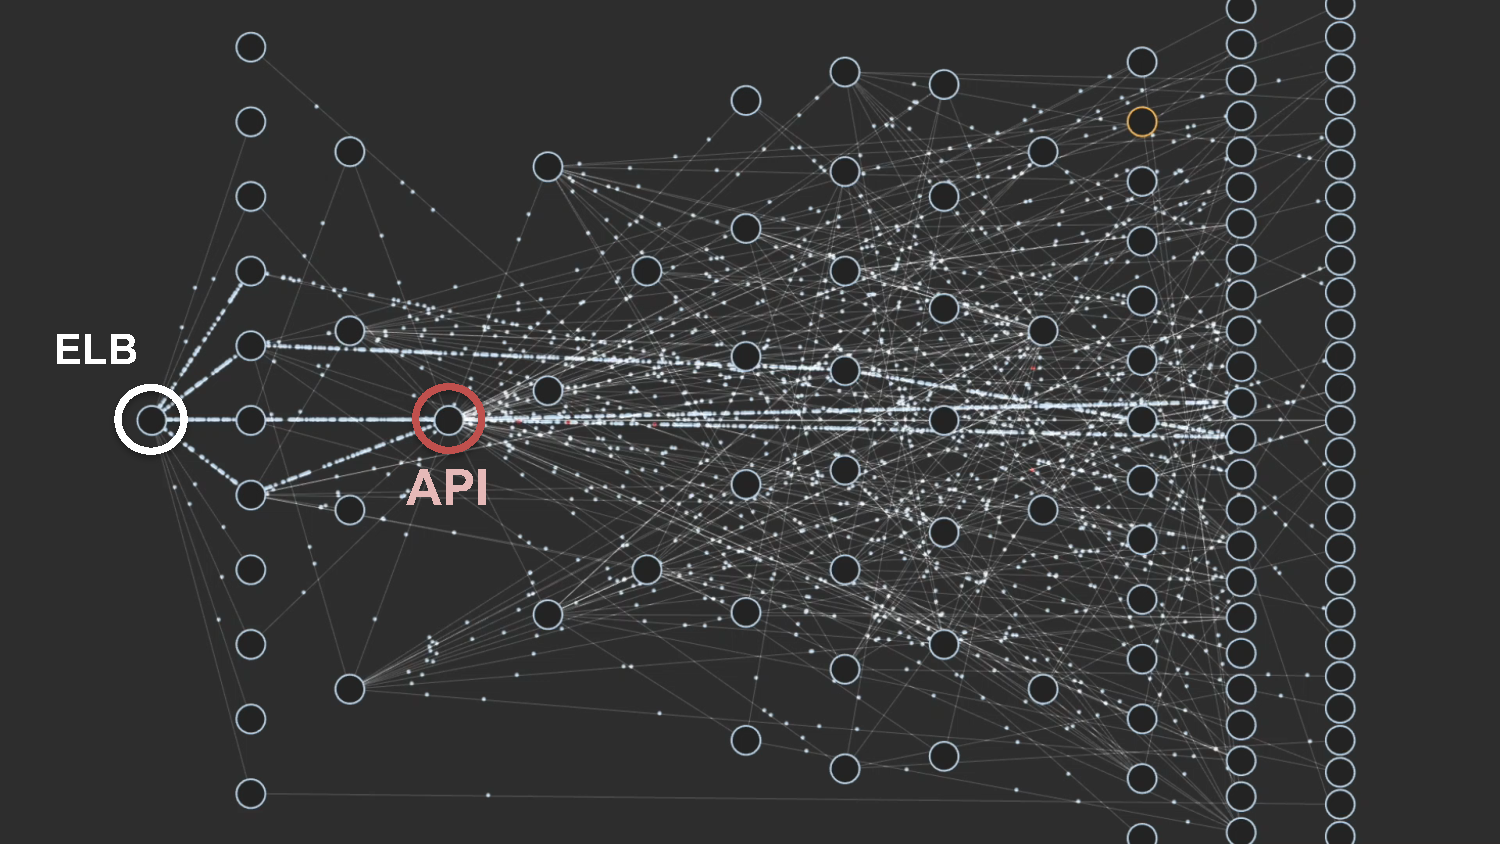
\includegraphics[width=\textwidth]{sources/Mastering Chaos.pdf}
		\end{center}
		\column{.3\textwidth} Josh Evans, CTO @ Netflix, QCon 2016 \cite*{JoshQCon}
	\end{columns}
\end{frame}

\begin{frame}{The Solution: Autonomous Management}
	\begin{columns}
		\column{.7\textwidth} \begin{center}
			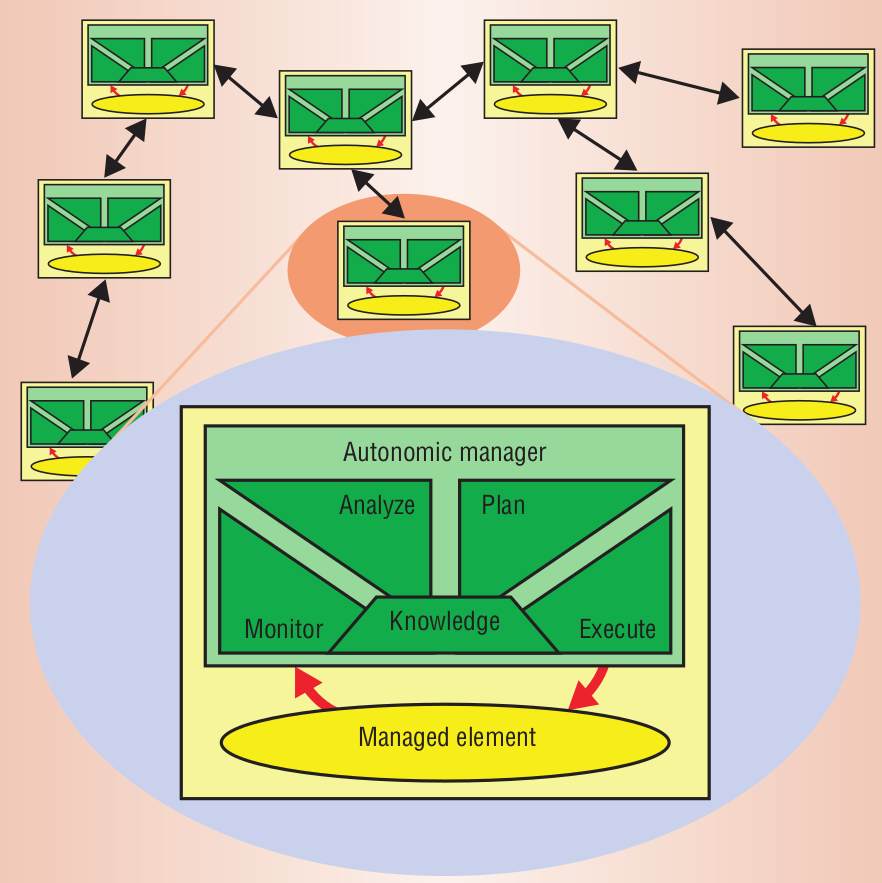
\includegraphics[height=0.7\textheight]{sources/MAPEK.png}
		\end{center}
		\column{.3\textwidth} \cite{VisionOfAutonomicComputing}
	\end{columns}
\end{frame}

\section{Self-Adaptive Systems}

\begin{frame}{Definition}
	\begin{greenblock}{Self-Adaptive System}
		A system which autonomously manages its self by:
		\begin{itemize}
			\item \textit{Monitoring} its environment,
			\item \textit{analyzing} changes
			\item \textit{planning} adaptations and
			\item \textit{executing} adaptations
		\end{itemize}
	\end{greenblock}
\end{frame}

\begin{frame}{Example: Online store}
	\begin{itemize}
		\item Scenario: System administrator of a commercial web service.
		\item Common task: Update system parameter X based on metric Y.
	\end{itemize}
	\medskip
	This can scenario can benefit from a Self-Adaptive System:
	\begin{itemize}
		\item Generalized adaptation rule:
		If metric Y crosses threshold Z: Update system parameter X.
		\item Example: If the server load gets too high: Start a new server instance.
	\end{itemize}
\end{frame}

\begin{frame}{Classifying Self-Adaptive Systems}
	\begin{columns}
		\column{.7\textwidth} \begin{center}
			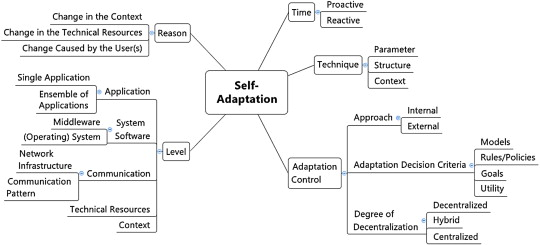
\includegraphics[width=\textwidth]{sources/KrupitzerTaxonomy.jpg}
		\end{center}
		\column{.3\textwidth} \cite{SurveyOnEngineeringApproaches}
	\end{columns}
\end{frame}

\begin{frame}{Limitations of Self-Adaptive Systems}
	\begin{center}
		\Large \textbf{Uncertainty}
		\\ \medskip
		Environment changes $\Rightarrow$ Unexpected adaptation results
	\end{center}
\end{frame}

\section{Optimization Approaches}

\begin{frame}{Optimizations for Self-Adaptive Systems}
	There is one main approach for optimizing Self-Adaptive Systems
	that is being used:
	\begin{itemize}
		\item Dynamically update adaptation rules.
	\end{itemize}
	\medskip
	In most cases machine learning is used to generate new adaptation rules
	or to update them. \\
	\medskip
	But other aspects can be optimized as well:
	\begin{itemize}
		\item Adaptation Control: How
		\item Level: Where
		\item Technique: What
	\end{itemize}
\end{frame}

\section{Classification Proposal}

\begin{frame}{Developing a classification}
	The classification is based on three concepts:
	\begin{itemize}
		\item Reflective computation (\cite{FORMS})
		\item The 5W+1H questions (\cite{LandscapeAndResearchChallenges})
		\begin{itemize}
			\item Who, What, Where, When, Why and How
		\end{itemize}
		\item The taxonomy for Self-Adaptive Systems (\cite{SurveyOnEngineeringApproaches})
	\end{itemize}
\end{frame}

\begin{frame}{Classification proposal}
	\begin{center}
		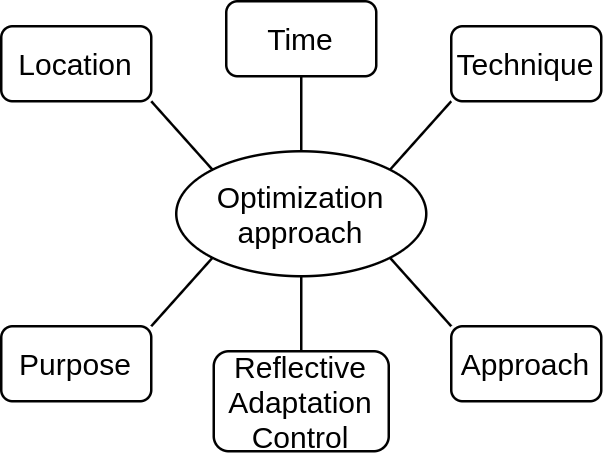
\includegraphics[width=.5\textwidth]{sources/ClassificationProposal-Proposal.png}
	\end{center}
\end{frame}

\begin{frame}{Classification proposal - Location}
	\begin{greenblock}{Location}
		\begin{itemize}
			\item Adaptation Control
			\item Level
			\item Technique
		\end{itemize}
	\end{greenblock}
\end{frame}

\begin{frame}{Classification proposal - Time}
	\begin{greenblock}{Time}
		\begin{itemize}
			\item Design time
			\item Run time / Online phase
			\item Offline phase
		\end{itemize}
	\end{greenblock}
\end{frame}

\begin{frame}{Classification proposal - Technique}
	\begin{greenblock}{Technique}
		\begin{itemize}
			\item Rules / Policies
			\item Knowledge
			\item Adaptation Technique
			\item Level
		\end{itemize}
	\end{greenblock}
\end{frame}

\begin{frame}{Classification proposal - Purpose}
	\begin{greenblock}{Purpose}
		\begin{itemize}
			\item Update Knowledge
			\item Apply Rules / Policies
			\item Goal Satisfaction
			\item Utility max-/minimization
		\end{itemize}
	\end{greenblock}
\end{frame}

\begin{frame}{Classification proposal - Approach}
	\begin{greenblock}{Approach}
		\begin{itemize}
			\item Internal / External
			\item Degree of decentralization:
			\begin{itemize}
				\item Fully centralized
				\item Fully decentralized
				\item Hybrid
			\end{itemize}
		\end{itemize}
	\end{greenblock}
\end{frame}

\begin{frame}{Classification proposal - Reflective Adaptation Control}
	\begin{greenblock}{Reflective Adaptation Control}
		\begin{itemize}
			\item Update Models
			\item Modify Rules / Policies
			\item Satisfy Goals
			\item Max-/Minimize Utilities
		\end{itemize}
	\end{greenblock}
\end{frame}

\begin{frame}{Classification proposal}
	\begin{center}
		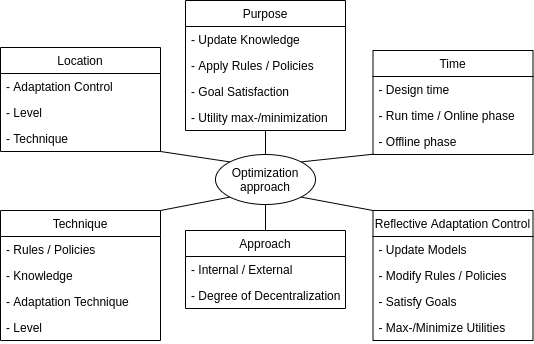
\includegraphics[width=.6\textwidth]{sources/ClassificationProposal-WithDimensions.png}
	\end{center}
\end{frame}

\section{Conclusion}

\begin{frame}{Conclusion}
	This field still requires further research:
	\begin{itemize}
		\item The proposed classification has to be applied to existing approaches.
		This could verify the classification and give a structured overview of the field.
		\item Different approaches need to be tested.
		For example: Optimization Approaches which focus on the Level or Technique.
		\item Most approaches that are currently used are highly domain specific.
		This applies to Self-Adaptive Systems and their Optimization Approaches.
	\end{itemize}
\end{frame}

\appendix
\beginbackup

\begin{frame}{Literatur}
\printbibliography
\end{frame}

\section{Farben}
%% ----------------------------------------
%% | Test-Folie mit definierten Farben |
%% ----------------------------------------
% \begin{frame}{Farbpalette}
% \tiny

% % GREEN
% 	\colorbox{kit-green100}{kit-green100}
% 	\colorbox{kit-green90}{kit-green90}
% 	\colorbox{kit-green80}{kit-green80}
% 	\colorbox{kit-green70}{kit-green70}
% 	\colorbox{kit-green60}{kit-green60}
% 	\colorbox{kit-green50}{kit-green50}
% 	\colorbox{kit-green40}{kit-green40}
% 	\colorbox{kit-green30}{kit-green30}
% 	\colorbox{kit-green25}{kit-green25}
% 	\colorbox{kit-green20}{kit-green20}
% 	\colorbox{kit-green15}{kit-green15}
% 	\colorbox{kit-green10}{kit-green10}
% 	\colorbox{kit-green5}{kit-green5}

% % BLUE
% 	\colorbox{kit-blue100}{kit-blue100}
% 	\colorbox{kit-blue90}{kit-blue90}
% 	\colorbox{kit-blue80}{kit-blue80}
% 	\colorbox{kit-blue70}{kit-blue70}
% 	\colorbox{kit-blue60}{kit-blue60}
% 	\colorbox{kit-blue50}{kit-blue50}
% 	\colorbox{kit-blue40}{kit-blue40}
% 	\colorbox{kit-blue30}{kit-blue30}
% 	\colorbox{kit-blue25}{kit-blue25}
% 	\colorbox{kit-blue20}{kit-blue20}
% 	\colorbox{kit-blue15}{kit-blue15}
% 	\colorbox{kit-blue10}{kit-blue10}
% 	\colorbox{kit-blue5}{kit-blue5}

% % RED
% 	\colorbox{kit-red100}{kit-red100}
% 	\colorbox{kit-red90}{kit-red90}
% 	\colorbox{kit-red80}{kit-red80}
% 	\colorbox{kit-red70}{kit-red70}
% 	\colorbox{kit-red60}{kit-red60}
% 	\colorbox{kit-red50}{kit-red50}
% 	\colorbox{kit-red40}{kit-red40}
% 	\colorbox{kit-red30}{kit-red30}
% 	\colorbox{kit-red25}{kit-red25}
% 	\colorbox{kit-red20}{kit-red20}
% 	\colorbox{kit-red15}{kit-red15}
% 	\colorbox{kit-red10}{kit-red10}
% 	\colorbox{kit-red5}{kit-red5}

% % GREY
% 	\colorbox{kit-gray100}{\color{white}kit-gray100}
% 	\colorbox{kit-gray90}{\color{white}kit-gray90}
% 	\colorbox{kit-gray80}{\color{white}kit-gray80}
% 	\colorbox{kit-gray70}{\color{white}kit-gray70}
% 	\colorbox{kit-gray60}{\color{white}kit-gray60}
% 	\colorbox{kit-gray50}{\color{white}kit-gray50}
% 	\colorbox{kit-gray40}{kit-gray40}
% 	\colorbox{kit-gray30}{kit-gray30}
% 	\colorbox{kit-gray25}{kit-gray25}
% 	\colorbox{kit-gray20}{kit-gray20}
% 	\colorbox{kit-gray15}{kit-gray15}
% 	\colorbox{kit-gray10}{kit-gray10}
% 	\colorbox{kit-gray5}{kit-gray5}

% % Orange
% 	\colorbox{kit-orange100}{kit-orange100}
% 	\colorbox{kit-orange90}{kit-orange90}
% 	\colorbox{kit-orange80}{kit-orange80}
% 	\colorbox{kit-orange70}{kit-orange70}
% 	\colorbox{kit-orange60}{kit-orange60}
% 	\colorbox{kit-orange50}{kit-orange50}
% 	\colorbox{kit-orange40}{kit-orange40}
% 	\colorbox{kit-orange30}{kit-orange30}
% 	\colorbox{kit-orange25}{kit-orange25}
% 	\colorbox{kit-orange20}{kit-orange20}
% 	\colorbox{kit-orange15}{kit-orange15}
% 	\colorbox{kit-orange10}{kit-orange10}
% 	\colorbox{kit-orange5}{kit-orange5}

% % lightgreen
% 	\colorbox{kit-lightgreen100}{kit-lightgreen100}
% 	\colorbox{kit-lightgreen90}{kit-lightgreen90}
% 	\colorbox{kit-lightgreen80}{kit-lightgreen80}
% 	\colorbox{kit-lightgreen70}{kit-lightgreen70}
% 	\colorbox{kit-lightgreen60}{kit-lightgreen60}
% 	\colorbox{kit-lightgreen50}{kit-lightgreen50}
% 	\colorbox{kit-lightgreen40}{kit-lightgreen40}
% 	\colorbox{kit-lightgreen30}{kit-lightgreen30}
% 	\colorbox{kit-lightgreen25}{kit-lightgreen25}
% 	\colorbox{kit-lightgreen20}{kit-lightgreen20}
% 	\colorbox{kit-lightgreen15}{kit-lightgreen15}
% 	\colorbox{kit-lightgreen10}{kit-lightgreen10}
% 	\colorbox{kit-lightgreen5}{kit-lightgreen5}

% % Brown
% 	\colorbox{kit-brown100}{kit-brown100}
% 	\colorbox{kit-brown90}{kit-brown90}
% 	\colorbox{kit-brown80}{kit-brown80}
% 	\colorbox{kit-brown70}{kit-brown70}
% 	\colorbox{kit-brown60}{kit-brown60}
% 	\colorbox{kit-brown50}{kit-brown50}
% 	\colorbox{kit-brown40}{kit-brown40}
% 	\colorbox{kit-brown30}{kit-brown30}
% 	\colorbox{kit-brown25}{kit-brown25}
% 	\colorbox{kit-brown20}{kit-brown20}
% 	\colorbox{kit-brown15}{kit-brown15}
% 	\colorbox{kit-brown10}{kit-brown10}
% 	\colorbox{kit-brown5}{kit-brown5}

% % Purple
% 	\colorbox{kit-purple100}{kit-purple100}
% 	\colorbox{kit-purple90}{kit-purple90}
% 	\colorbox{kit-purple80}{kit-purple80}
% 	\colorbox{kit-purple70}{kit-purple70}
% 	\colorbox{kit-purple60}{kit-purple60}
% 	\colorbox{kit-purple50}{kit-purple50}
% 	\colorbox{kit-purple40}{kit-purple40}
% 	\colorbox{kit-purple30}{kit-purple30}
% 	\colorbox{kit-purple25}{kit-purple25}
% 	\colorbox{kit-purple20}{kit-purple20}
% 	\colorbox{kit-purple15}{kit-purple15}
% 	\colorbox{kit-purple10}{kit-purple10}
% 	\colorbox{kit-purple5}{kit-purple5}

% % Cyan
% 	\colorbox{kit-cyan100}{kit-cyan100}
% 	\colorbox{kit-cyan90}{kit-cyan90}
% 	\colorbox{kit-cyan80}{kit-cyan80}
% 	\colorbox{kit-cyan70}{kit-cyan70}
% 	\colorbox{kit-cyan60}{kit-cyan60}
% 	\colorbox{kit-cyan50}{kit-cyan50}
% 	\colorbox{kit-cyan40}{kit-cyan40}
% 	\colorbox{kit-cyan30}{kit-cyan30}
% 	\colorbox{kit-cyan25}{kit-cyan25}
% 	\colorbox{kit-cyan20}{kit-cyan20}
% 	\colorbox{kit-cyan15}{kit-cyan15}
% 	\colorbox{kit-cyan10}{kit-cyan10}
% 	\colorbox{kit-cyan5}{kit-cyan5}
		
% \end{frame}
% %% ----------------------------------------
% %% | /Test-Folie mit definierten Farben |
% %% ----------------------------------------
\backupend

\end{document}